\documentclass{article}

\usepackage[a4paper, total={6in, 10in}]{geometry}
\usepackage{tikz}
\usetikzlibrary{shapes.geometric, arrows}

%Flowchart Setup
\tikzstyle{boxes} = [rectangle, minimum width=2cm, minimum height=1cm, text centered, text
width=2cm, draw=black]
\tikzstyle{arrow} = [thick, ->, >=stealth]
\tikzstyle{infobox} = [trapezium, trapezium left angle=70, trapezium right angle=110, minimum
width=2cm, minimum height=1cm, text centered, text width=2cm, draw=black]

\title{Brad Flavall Guest Lecture Summary}

\author{Jos Craw\\35046080}

\begin{document}

\maketitle{}

Brad's lecture was on industry structure. He works at Beca where he worked on an indoor substation
in Christchurch. First Brad talked about the New Zealand power distribution network and its
various stages.\\

\begin{figure}[h]
%Drawing flowchart
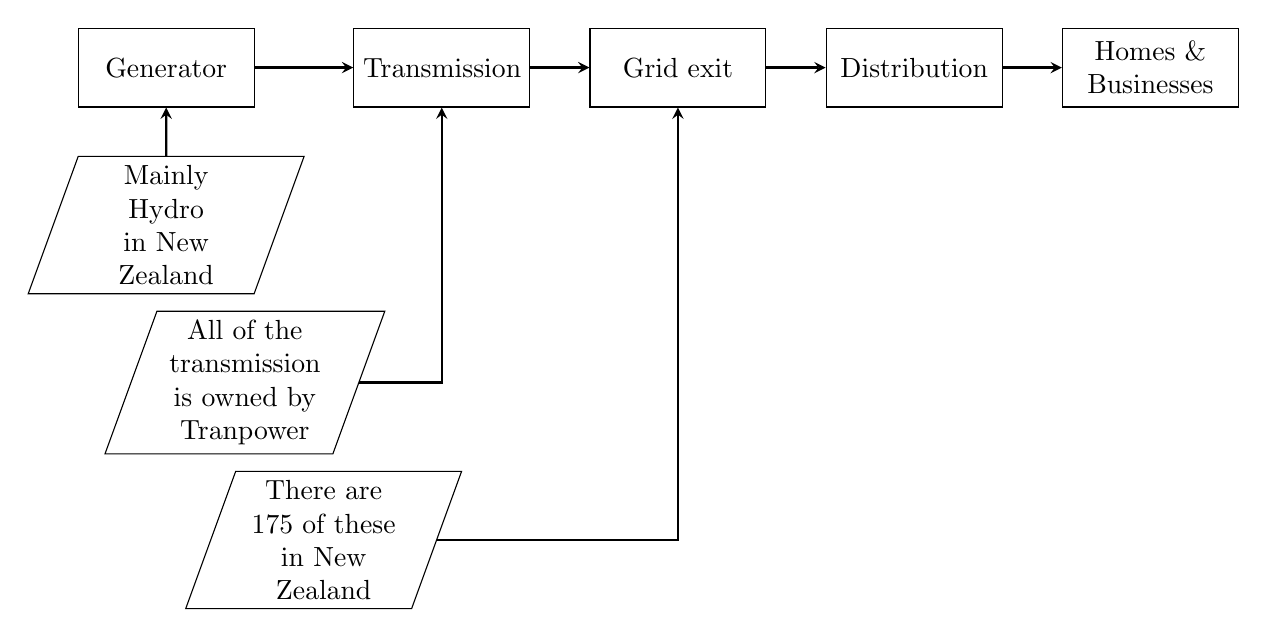
\begin{tikzpicture}
    %Main Nodes
    \node (gen) [boxes] {Generator};
    \node (trans) [boxes, right of=gen, xshift=2.5cm] {Transmission};
    \node (gridEx) [boxes, right of=trans, xshift=2cm] {Grid exit};
    \node (dist) [boxes, right of=gridEx, xshift=2cm] {Distribution};
    \node (output) [boxes, right of=dist, xshift=2cm] {Homes \& Businesses};

    %Supplementary Nodes
    \node (genInfo) [infobox, below of=gen, yshift=-1cm] {Mainly Hydro in New Zealand};
    \node (transInfo) [infobox, below of=trans, right of=genInfo, yshift=-1cm] {All of the transmission is owned by Tranpower};
    \node (gridExInfo) [infobox, below of=gridEx, right of=transInfo, yshift=-1cm] {There are 175 of these in New Zealand};

    %Arrows
    \draw [arrow] (gen) -- (trans);
    \draw [arrow] (trans) -- (gridEx);
    \draw [arrow] (gridEx) -- (dist);
    \draw [arrow] (dist) -- (output);
    \draw [arrow] (genInfo) -- (gen);
    \draw [arrow] (transInfo) -| (trans);
    \draw [arrow] (gridExInfo) -| (gridEx);
    
\end{tikzpicture}
\caption{The New Zealand power distribution network}
\end{figure}

\end{document}
